% 格式基本参照研究生学位论文撰写格式的统一要求,正文为小四号宋体

\documentclass[UTF-8,a4paper,twoside]{article}

% \author{blanche}

\usepackage[UTF8,heading = true]{ctex}
\usepackage{setspace}
\usepackage{fancyhdr}
\usepackage{enumitem}
\setlist[enumerate]{label=(\arabic*),fullwidth,itemindent=\parindent,listparindent=\parindent,itemsep=0ex,partopsep=0pt,parsep=0ex,nosep} % 列表标号加括号,取消缩进和前后间距
\raggedbottom % 禁用页面对齐调整
\usepackage{lastpage}
\usepackage{layout}
\usepackage{geometry}
\usepackage{graphicx}
\usepackage{subfig}
% 解决兼容性报错
\makeatletter
\let\c@lofdepth\relax
\let\c@lotdepth\relax
\makeatother
\usepackage{listings}

\usepackage{float}
\usepackage{abstract}
\usepackage[backend=biber,style=gb7714-2015,gbalign=left,gbnamefmt=lowercase]{biblatex}
\addbibresource{bib_template.bib}
\renewcommand{\bibfont}{\zihao{-4}} % 修改参考文献字号
\setlength{\bibitemsep}{0pt} % 去掉参考文献段间距
% 设置会议期刊名首字母大写,并去除其中的一些介词
\usepackage{mfirstuc}
\gMFUnocap{in}
\gMFUnocap{of}
\gMFUnocap{and}
\gMFUnocap{for}
\gMFUnocap{the}
\gMFUnocap{th}
\gMFUnocap{on}
\DeclareFieldFormat[article]{journaltitle}{\capitalisewords{#1}}
\DeclareFieldFormat[inproceedings]{booktitle}{\capitalisewords{#1}}


\AtBeginDocument{
\setlength{\abovedisplayskip}{1ex} % 设置公式前的垂直间距为零
\setlength{\belowdisplayskip}{1ex} % 设置公式后的垂直间距为零
}

\usepackage{fontspec}
\usepackage{caption}
\captionsetup[figure]{belowskip=-2ex} % 设置图片标题与后文垂直间距
\usepackage{bicaption}
% \setmainfont{TimesNewRomanPSMT}
\usepackage{newtxtext} % 设置全局Times New Roman字体
\usepackage{amsmath,lmodern}
\usepackage{xeCJK}
\usepackage{titletoc}
\usepackage{tocloft}
\usepackage{bm}
\usepackage{booktabs}%三线表

\newcommand{\topline}{\toprule[1.5pt]}	%三线表顶部线宽
\newcommand{\bottomline}{\bottomrule[1.5pt]}	%三线表底部线宽
\renewcommand{\contentsname}{\zihao{4}\bfseries{目录}}
\setlength{\cftsecindent}{0em}
\setlength{\cftsubsecindent}{0em}
\setlength{\cftsubsubsecindent}{0em}
\setlength{\cftbeforetoctitleskip}{1em}
\setlength{\cftaftertoctitleskip}{2em}
\renewcommand{\cftdotsep}{0.5}	% 目录引导线点间距

\renewcommand{\cftsecfont}{\zihao{4}}
\renewcommand{\cftsecpagefont}{\zihao{4}}
\renewcommand{\cftsubsecfont}{\zihao{-4}}
\renewcommand{\cftsubsubsecfont}{\zihao{-4}}
\renewcommand{\cftsecleader}{\cftdotfill{\cftdotsep}}
\setlength{\cftbeforesecskip}{0em}  %对目录格式进行修改
\setlength{\cftbeforesubsecskip}{0em}  %对目录格式进行修改
\setlength{\cftbeforesubsubsecskip}{0em}  %对目录格式进行修改



\numberwithin{equation}{section} % 公式按章节编号
\numberwithin{table}{section} % 表按章节编号
\numberwithin{figure}{section} % 图按章节编号
\renewcommand{\theequation}{\thesection-\arabic{equation}} % 连接符改为-
% 使用中文括号
% \renewcommand{\eqref}[1]{\textup{(\ref{#1})}}
\DeclareCaptionLabelSeparator{colon}{ \ \ } % 表连接符改为两个空格
\DeclareCaptionFont{chfont}{\bfseries\zihao{5}} % 表题宋体加粗五号
\DeclareCaptionFont{enfont}{\zihao{5}} % 表题宋体加粗五号
\captionsetup[table]{font=chfont}
\captionsetup[table][bi-second]{name=Table, font=enfont}
\captionsetup[figure]{font=chfont}
\captionsetup[figure][bi-second]{name=Fig., font=enfont}
% 重新定义 subfloat 标题的格式
\DeclareCaptionFont{subfont}{\zihao{5}} % 表题宋体加粗五号
\captionsetup[subfloat]{font=subfont}


% 页边距
\geometry{left=2.5cm,right=2.5cm,top=2.8cm,bottom=2.0cm,headheight=2.0cm,footskip=1.2cm}
% \setCJKfamilyfont{times}{Times New Roman} % 设置英文字体
\setCJKmainfont{SimSun.ttc}[AutoFakeBold=true, Path=./SimSun/, Extension = .ttc] % 设置宋体伪粗体
\let\kaishu\relax
\newCJKfontfamily\kaishu{SimKai.ttf}[AutoFakeBold=true, Path=./KaiTi/, Extension= .ttf] % 设置楷体伪粗体

% 更改章节标题样式
\ctexset{
	section={
	name={第,章},
	format=\heiti\zihao{4}\centering,
	beforeskip=3ex,
	afterskip=3ex
	},
	subsection={
	format=\bfseries\zihao{-4},
	beforeskip=0.6em,
	afterskip=0.6em
	},
	subsubsection={
	format=\zihao{-4},
	beforeskip=0ex,
	afterskip=0ex
	}
}

% 设置段落间距
\usepackage{parskip}
\setlength{\parskip}{0pt}
\setlength{\parindent}{2em}
% 正文页
\fancypagestyle{main}{
\fancyhf{}
\linespread{1.4375} % 1.25倍行距
\fancyhead[LO,RE]{\kaishu\bfseries\zihao{4}{华东理工大学}\normalfont\songti\zihao{-4}{硕士学位论文}}
\fancyhead[RO,LE]{\zihao{-4}{第}\thepage{页}}
}

% 扉页
\fancypagestyle{pre}{
\fancyhf{}
\linespread{1.4375} % 1.25倍行距
\fancyhead[LO,RE]{\kaishu\bfseries\zihao{4}{华东理工大学}\normalfont\songti\zihao{-4}{硕士学位论文}}
\fancyhead[RO,LE]{\zihao{-4}{第}\Roman{page}{页}}
}

\begin{document}

\pagestyle{pre}
\thispagestyle{pre}
\begin{center}
	\heiti\zihao{4}论文题目
\end{center}
\vspace{\baselineskip}
\begin{center}
	\zihao{4}\bfseries{摘要}
\end{center}

\zihao{-4}摘要摘要摘要摘要摘要摘要摘要摘要摘要摘要摘要摘要摘要摘要摘要摘要摘要摘要摘要摘要摘要摘要摘要摘要摘要摘要摘要摘要摘要摘要摘要摘要摘要摘要摘要摘要摘要摘要摘要摘要。

本文的主要工作包括:

\begin{enumerate}[itemsep=0pt,topsep=0pt]
	\item 针对摘要摘要摘要摘要摘要摘要摘要摘要摘要摘要摘要摘要摘要摘要摘要摘要摘要摘要摘要摘要摘要摘要摘要摘要摘要摘要摘要摘要摘要摘要摘要摘要摘要摘要摘要摘要摘要摘要。
	\item 摘要摘要摘要摘要摘要摘要摘要摘要摘要摘要摘要摘要摘要摘要摘要摘要摘要摘要摘要摘要摘要摘要。
	\item 摘要摘要摘要摘要摘要摘要摘要摘要摘要摘要摘要摘要摘要摘要摘要摘要摘要摘要摘要摘要摘要摘要。
\end{enumerate}

综上所述,摘要摘要摘要摘要摘要摘要摘要摘要摘要摘要摘要摘要摘要摘要摘要摘要摘要摘要摘要摘要摘要摘要摘要摘要摘要摘要摘要摘要摘要摘要摘要摘要摘要摘要摘要摘要。

\noindent\zihao{-4}{\bfseries 关键词:}深度学习;xxx;xxx;xxx

\newpage
\begin{center}
	\zihao{4}\bfseries Your Thesis Title in English
\end{center}
\vspace{\baselineskip}

\begin{center}
	\zihao{4}\bfseries{Abstract}
\end{center}

\zihao{-4}
Abstract abstract abstract.

The main work of this thesis includes:

\begin{enumerate}[itemsep=0pt,topsep=0pt]
\item We use xxxx to xxxx.
\item For xxx.
\item xxxx.
\end{enumerate}

In summary, abstract abstract abstract abstract abstract abstract abstract abstract abstract abstract abstract abstract abstract abstract.

\noindent\zihao{-4}{\bfseries Keywords \ \ }Deep learning; xxx; xxx; xxx
%\end{abstract}

% 目录
\newpage
\thispagestyle{pre}
\tocloftpagestyle{pre}
\begin{center}
	\tableofcontents
\end{center}
\thispagestyle{pre}

\newpage
\pagestyle{main}
\setcounter{page}{1}
\section{绪论}
绪论绪论绪论绪论绪论绪论绪论绪论绪论绪论绪论绪论绪论绪论绪论绪论绪论。本章将绪论绪论绪论绪论绪论绪论绪论绪论绪论绪论绪论绪论绪论绪论绪论绪论绪论绪论绪论绪论绪论绪论。

\subsection{研究背景及意义}
\zihao{-4}
由于绪论\cite{cbam}绪论绪论绪论绪论绪论绪论绪论绪论绪论绪论\cite{公安联网标准}绪论绪论绪论绪论绪论绪论绪论绪论绪论绪论绪论绪论绪论绪论绪论绪论绪论。

\subsection{国内外研究现状}
本课题涉及绪论绪论绪论\cite{廖云飞}绪论绪论绪论绪论绪论绪论绪论绪论绪论\cite{渣土车未苫盖检测}绪论绪论绪论绪论绪论绪论绪论绪论绪论绪论绪论绪论绪论绪论绪论绪论绪论绪论。

\subsubsection{相关研究}
绪论绪论绪论绪论绪论绪论绪论绪论\cite{duchi2011adaptive}绪论绪论绪论绪论绪论绪论绪论绪论绪论绪论绪论\cite{kingma2014adam}绪论绪论绪论绪论绪论绪论绪论绪论绪论绪论绪论绪论绪论。

\newpage
\section{理论基础}
理论基础理论基础理论基础理论基础理论基础理\cite{lee2021mlcourse}论基础理论基础理论基础理论基础理论基础理论基础理论基础理论基础理论基础理论基础理论基础理论基础理论基础理论基础。

\subsection{方法}
方法方法方法方法方法方法方法方法方法方法方法方法方法\cite{mobilenet}方法方法方法方法方法方法\cite{wang2020cspnet,mobilenet}方法方法方法。

如图\ref{f1}所示。
\begin{figure}[!h]
	\centering
	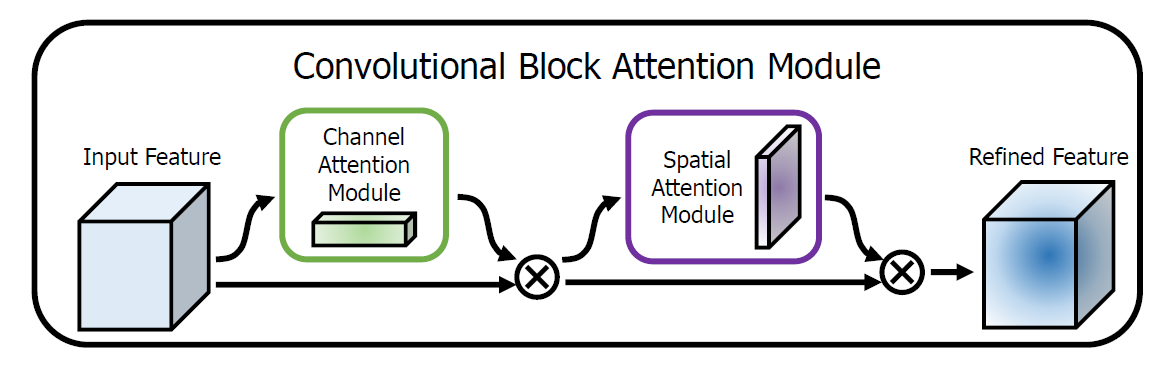
\includegraphics[width=0.6\textwidth]{cbam1.png}
	\bicaption{图像示例}{Examples of xxx}
	\label{f1}
\end{figure}

如图\ref{f2}所示,子图如图\ref{f2:a}所示。
\begin{figure}[!h]
	\centering
	\subfloat[baseline\label{f2:a}]{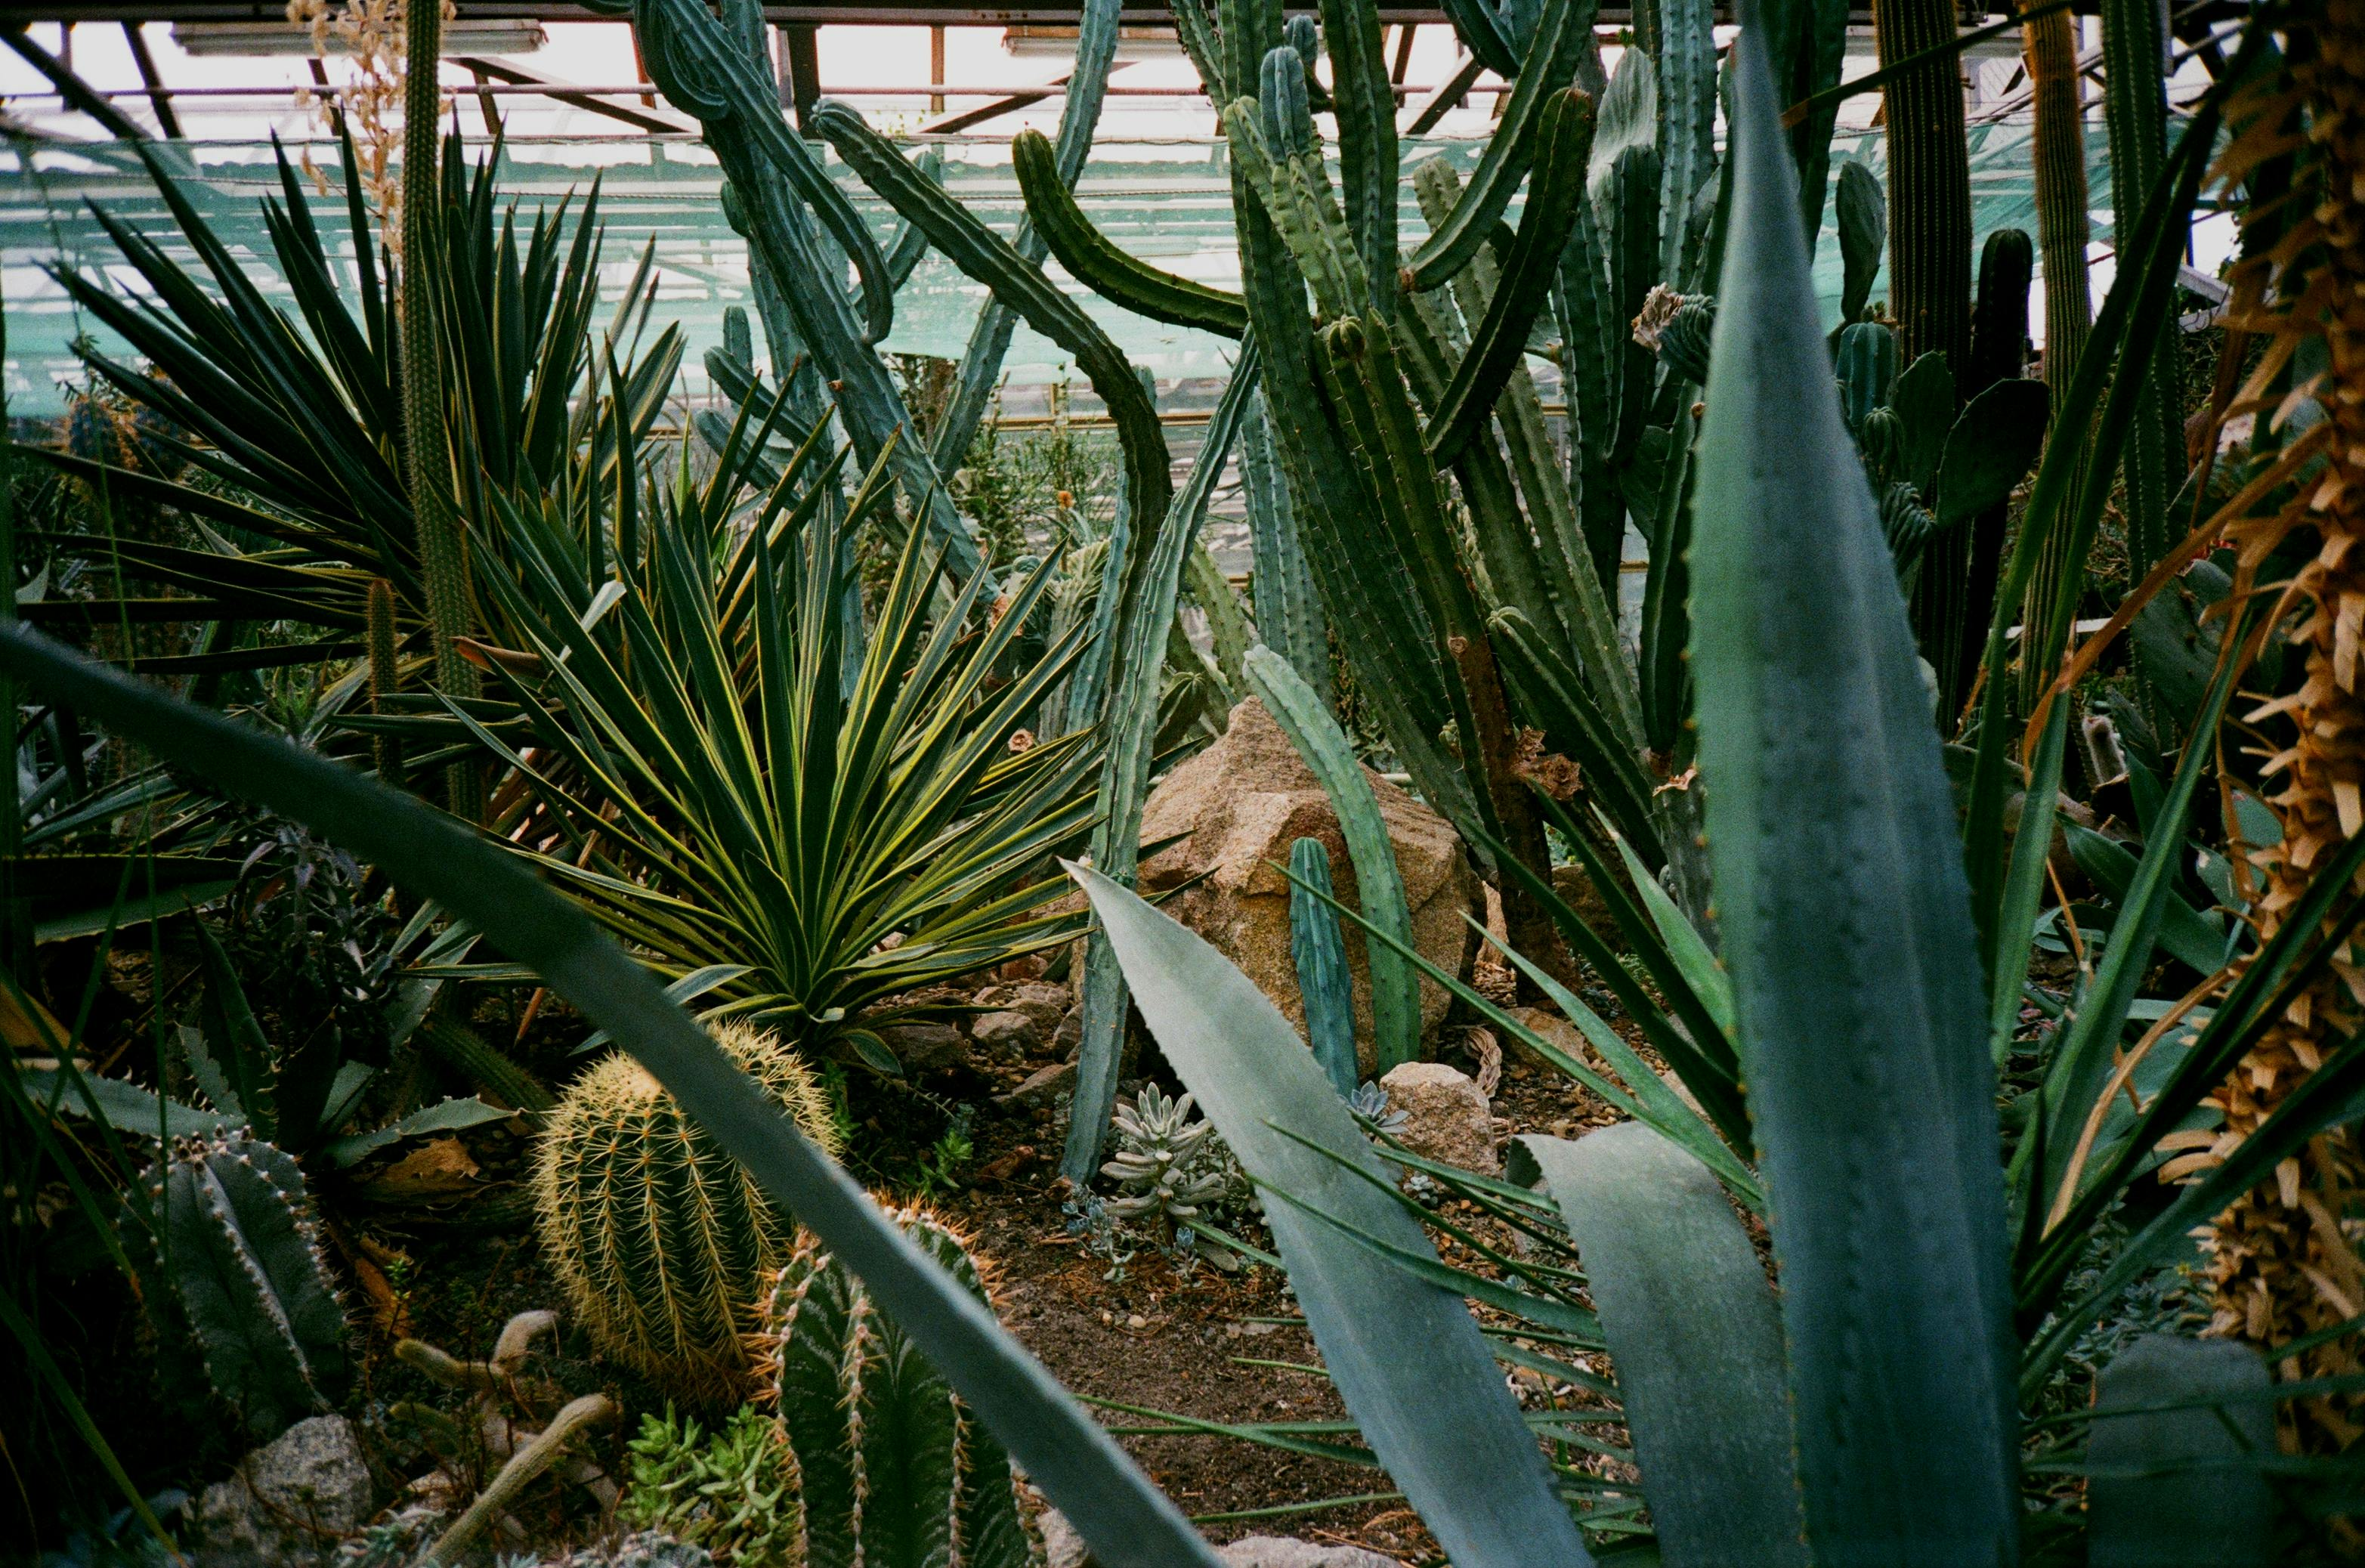
\includegraphics[width=0.45\textwidth]{eg1.jpg}}\\
	\subfloat[ours]{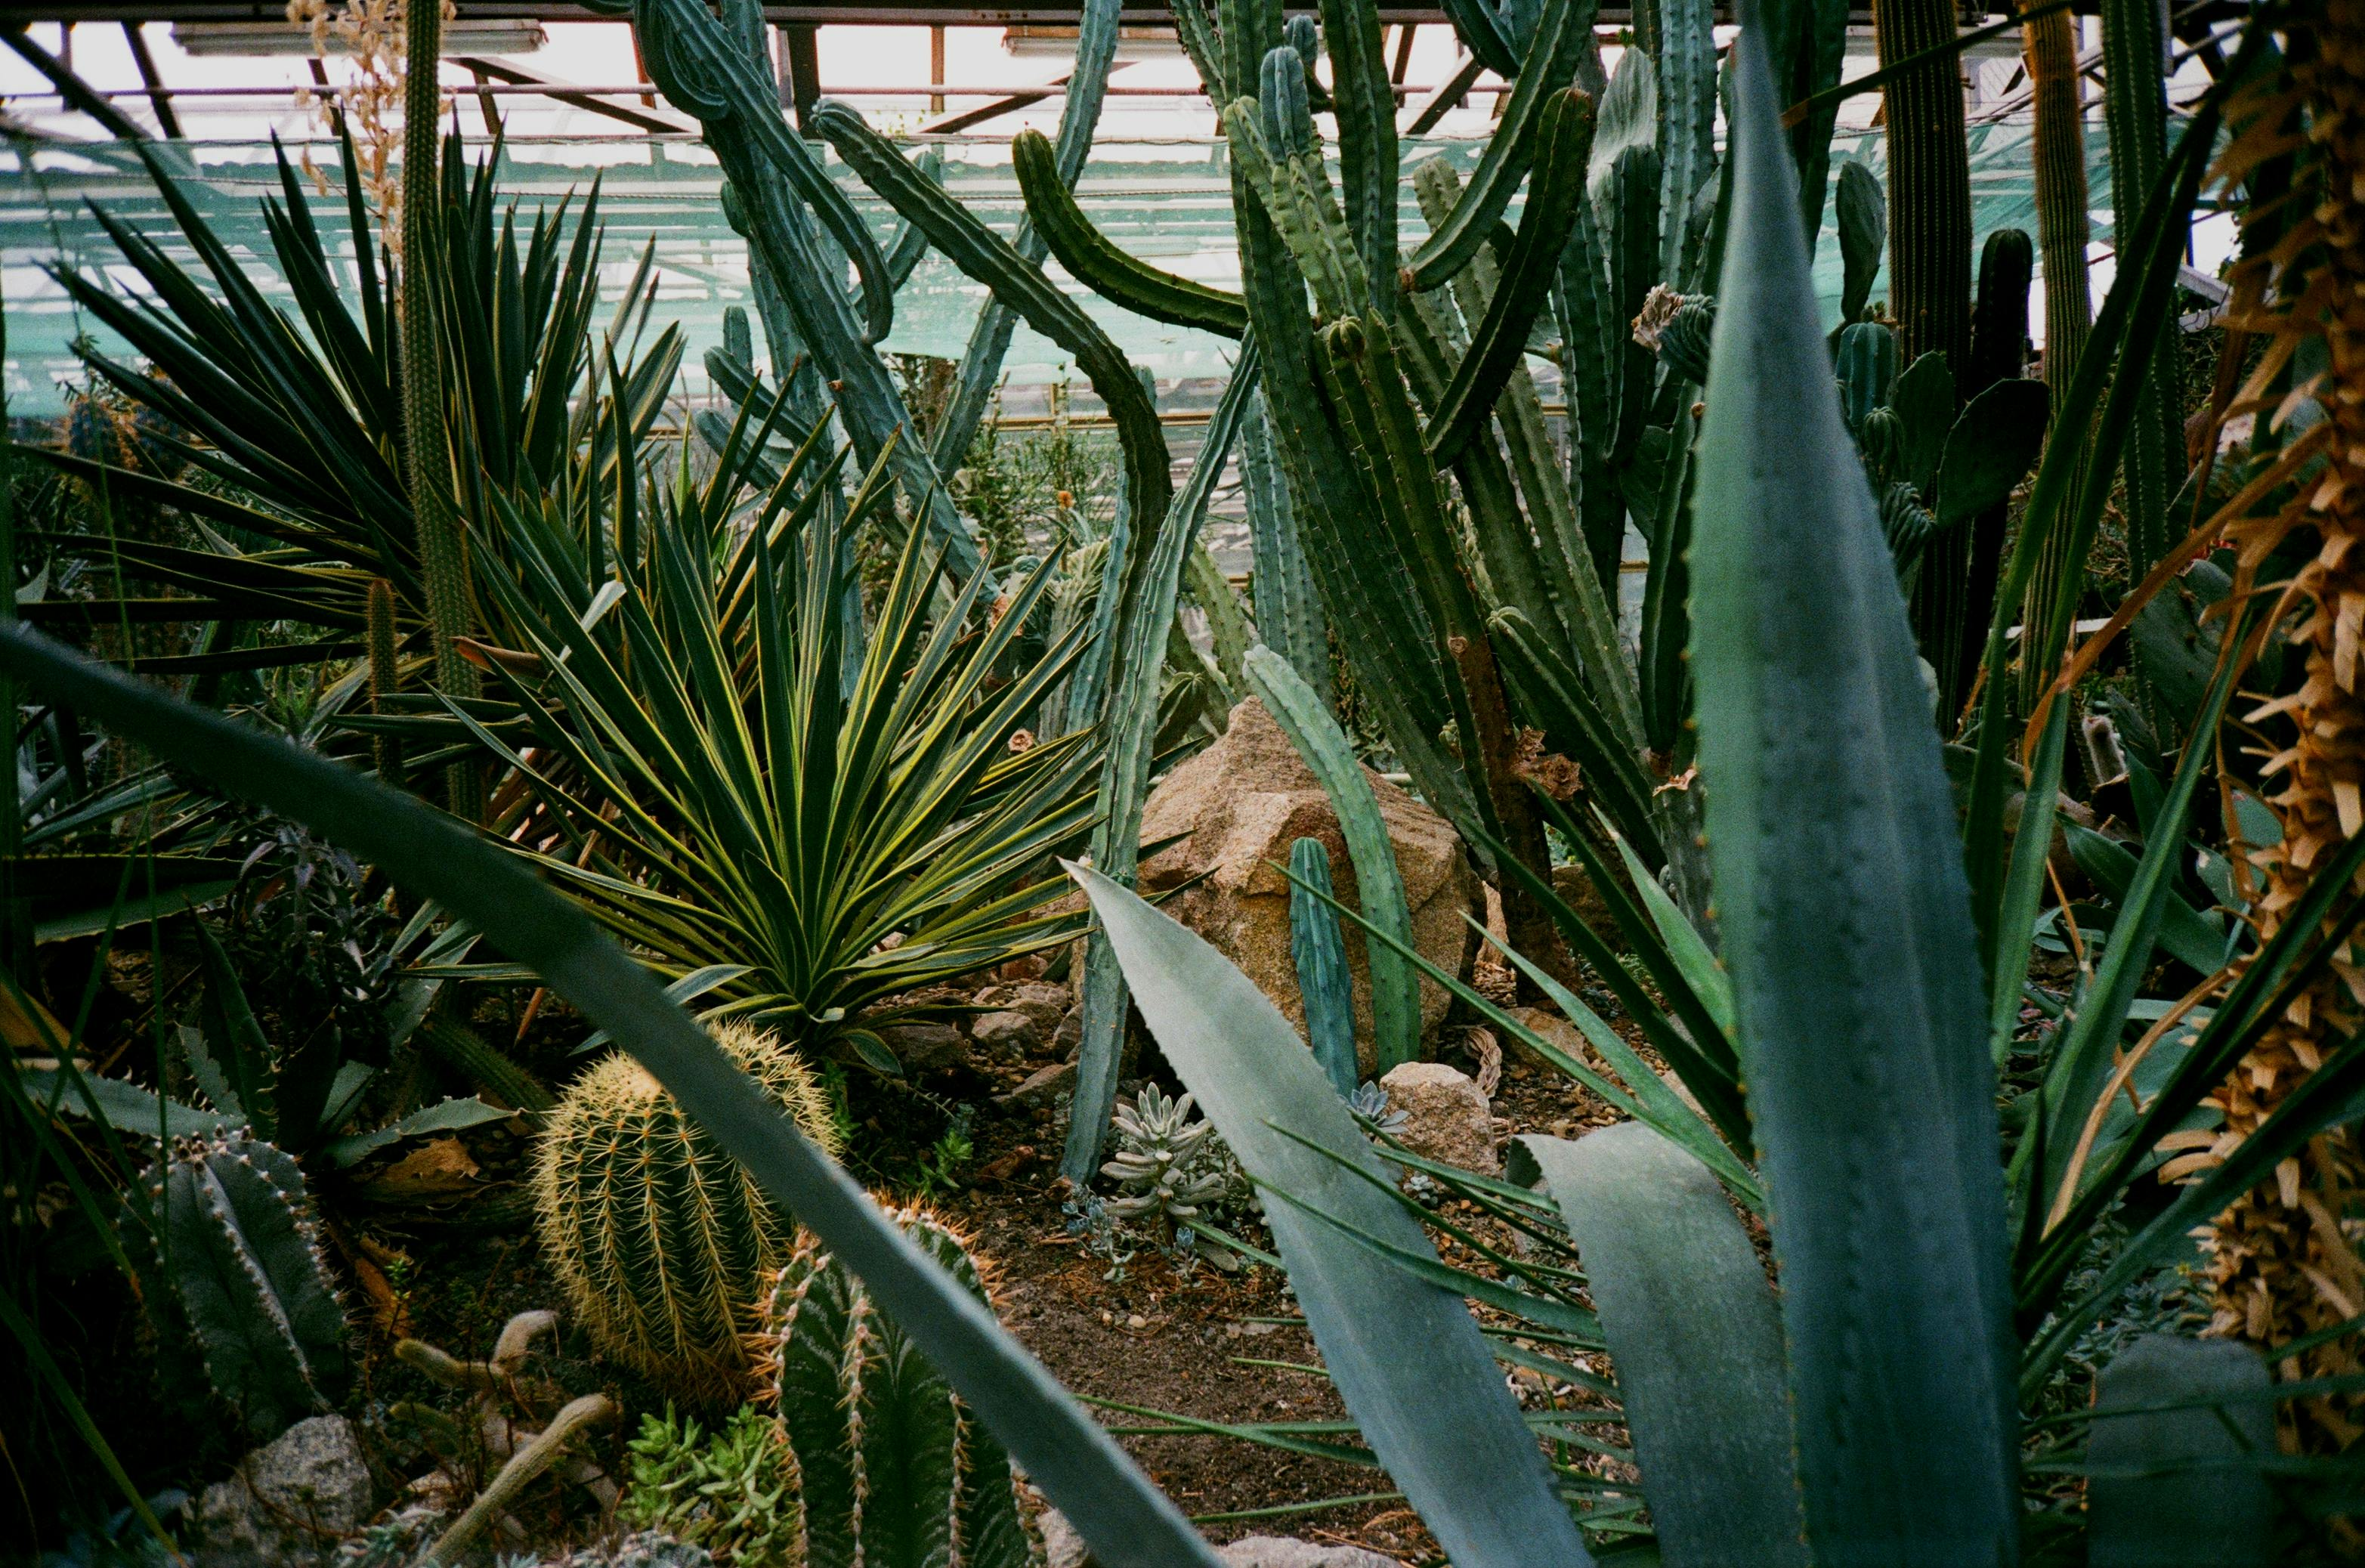
\includegraphics[width=0.45\textwidth]{eg1.jpg}}\\
	\bicaption{图片示例}{Examples}
	\label{f2}
\end{figure}

YOLOv5采用的激活函数是SiLU函数,公式如式\eqref{e1}所示。式中,$x$表示输入,$f(x)$表示输出,$\sigma(x)$表示Sigmoid函数。
\begin{subequations}
  \label{e1}
  \begin{align}
    f(x)      & = x \cdot \sigma(x)    \\
    \sigma(x) & = \frac{1}{1 + e^{-x}}
  \end{align}
\end{subequations}

\newpage
\section{XXX模型}
\subsection{模型训练和改进}
表\ref{t1}展示了……
\begin{table}[!h]
	\centering
	\bicaption{基线模型测试结果}{The baseline result of xxx test}
	\label{t1}
	\begin{tabular}{c c c c c c}
		\topline
		\text{类别}                & \text{目标框数量} & \text{Precision} & \text{Recall} & \text{AP} & \text{F1-score} \\
		\midrule
		car                      & xx       & xx           & xx        & xx    & xx          \\

		van                      & xx         & xx           & xx        & 0.73    & xx          \\

		bus                      & xx          & 0.8           & xx        & xx    & xx          \\
		\bottomline
	\end{tabular}
\end{table}

\newpage
\addcontentsline{toc}{section}{参考文献}
% \zihao{-4}\bibliography{paper_version1}
\defbibheading{bibliography}[\bibname]{\section*{#1}\bfseries\zihao{4}\heiti\normalfont} % 参考文献标题格式

\printbibliography[heading=bibliography,title=参考文献]

\newpage
\addcontentsline{toc}{section}{致谢}
\begin{center}
	\zihao{4}\bfseries{致谢}
\end{center}
\vspace{\baselineskip}

\zihao{-4}{此篇论文完稿之际,首先要感谢致谢致谢致谢致谢致谢致谢致谢致谢致谢致谢致谢致谢致谢致谢致谢致谢致谢致谢致谢致谢致谢致谢致谢致谢致谢致谢致谢致谢致谢致谢致谢致谢致谢致谢。}

\end{document}